\documentclass[c]{beamer}
\mode<presentation>
{
  \usetheme[progressbar=frametitle]{metropolis}
  \usecolortheme{default}
  \usefonttheme{serif}
  \setbeamertemplate{navigation symbols}{}
  \setbeamertemplate{caption}[numbered]
  \setbeamercovered{transparent}
}
\addtobeamertemplate{block begin}{\pgfsetfillopacity{0.8}}{\pgfsetfillopacity{1}}
\addtobeamertemplate{block alerted begin}{\pgfsetfillopacity{0.8}}{\pgfsetfillopacity{1}}
\addtobeamertemplate{block example begin}{\pgfsetfillopacity{0.8}}{\pgfsetfillopacity{1}}

\usepackage[T1]{fontenc}
\usepackage[utf8]{inputenc}
\usepackage[brazil]{babel}
\usepackage[brazilian,hyperpageref]{backref}
\usepackage[scale=2]{ccicons}
\usepackage{pgfplots}
\usepackage{braket}
\usepackage{cancel}
\usepackage{mathtext}
\usepackage{amsfonts,amssymb}
\usepackage{amsmath,amsthm}
\usepackage{epsfig,epstopdf,url,array,latexsym}
\usepackage{graphicx}
\usepackage{mathrsfs}
\usepackage{natbib}
\usepackage{float}
\usepackage{caption}
\usepackage{subcaption}
\usepackage[mathcal]{euscript}
\usepackage{esvect}
\captionsetup[figure]{labelfont=sc}
\usepackage{microtype} 
\usepackage{multicol}
\usepackage{multirow}
\usepackage{longtable}
\usepackage{lscape}
\usepackage{booktabs}
\usepackage{verbatim}
\usepackage{cprotect}
\usepackage{xpatch}
\usepackage{ragged2e}
\usepackage{etoolbox}
\usepackage{comment}

\title{
    {\sc Introdução ao \LaTeX}
    }
\subtitle{Módulo I: o básico + texto}
\date{13/11/2023 e 14/11/2023}
\author{
    {\large Introdução ao \LaTeX}\\[0.3cm]
	Lucas {\sc Gregolon} \inst{1}
	\footnote{\href{FisicaComOGreg@gmail.com}{\texttt{FisicaComOGreg@gmail.com}}}
	}
\institute{
    {\inst{1} \large Instituto de Matemática, Estatística e Física - IMEF/FURG}\\[0.2cm]
    }
\titlegraphic{
    \hfill          
\includegraphics[height=1.9cm]{images/furg.png}
                    %
\includegraphics[height=2.0cm]{images/ufpel.png}\\[4.8cm]
	%\hspace*{8.1cm}   
\includegraphics[height=2.0cm]{images/latexcomcafe.jpg}
    }

\newcommand{\themename}{\textbf{\textsc{metropolis}}\xspace}
\newcommand{\qv}[1]{\widetilde{#1}}
\renewcommand{\r}{\right}
\renewcommand{\l}{\left}
\newcommand*{\EE}{\mathscr{E}}
\newcommand*{\BB}{\mathscr{B}}
\newcommand*{\Hh}{\mathscr{H}}
\newcommand*{\D}{{\rm d}}
\newcommand*{\PP}{\mathscr{P}}
\newcommand*{\WW}{\mathcal{W}}
\newcommand*{\A}{\mathscr{A}}
\newcommand*{\ii}{\mathfrak{i}}
\newcommand{\source}[1]{
    \caption*{Fonte: {#1}} 
    }
\bibliographystyle{apalike}
\setbeamertemplate{section in toc}{\hspace*{1em}\inserttocsectionnumber.~\inserttocsection\par}
\setbeamertemplate{subsection in toc}{\hspace*{2em}\inserttocsectionnumber.\inserttocsubsectionnumber.~\inserttocsubsection\par}
\setbeamercovered{invisible}
\apptocmd{\frame}{}{\justifying}{}

\begin{document}

\maketitle

{
\fontsize{9pt}{10.0}\selectfont

\begin{frame}[fragile]{\sc Sumário}
    
	\begin{multicols}{2}
	    \tableofcontents
	\end{multicols}
	
\end{frame}
}

{
\fontsize{10pt}{10.0}\selectfont

\begin{comment}
    
    \begin{frame}[fragile]{\sc Resumo}
    
    \begin{itemize}
        
        \item \LaTeX \ é um editor de textos de alta qualidade tipográfica e de robusta formatação.
        \item Vem sendo muito utilizado pela academia científica mas esta se estendendo a mais áreas do conhecimento. O minicurso tem o objetivo de introduzir a linguagem LaTeX, expondo sua estrutura básica, os principais comandos utilizados, o ambiente matemático e como criar e  lidar com citações e referências bibliográficas. Também será mostrado como criar e editar uma apresentação no ambiente ``beamer'' (análogo ao Power Point).
        \item Além disso, o minicurso fornecerá um panorama geral de maneiras para se produzir documentos científicos, tais como artigos e livros, no formato padrão das revistas de publicações.
        \item Espera-se que no final do minicurso, os alunos tenham adquirido uma ideia geral do funcionamento do \LaTeX \ e que estejam aptos a criar documentos e apresentações com fórmulas matemáticas e controle de referências.
        
    \end{itemize}
    
\end{frame}
    
\end{comment}

\section{Motivação}
    
    \begin{frame}[standout]
        
        Por que utilizar o \LaTeX \ como editor de texto?
        
    \end{frame}

    \begin{frame}[fragile]{\sc Vantagens}
        
	    \begin{itemize}
        \setlength\itemsep{0.2cm}
            
		    \item O \LaTeX\ permite a {\color{blue} criação} e {\color{blue} edição} de textos em variadas maneiras;
		    \item Possui uma alta {\color{blue} qualidade tipográfica};
		    \item É eficiente na {\color{blue} organização do texto} quando ele é complexo ou grande;
		    \item É a melhor ferramenta para quem precisa {\color{blue} escrever equações} (Física, Matemática, Estatística, Economia, ...);
		    \item Além disso, é muito útil para quem não trabalha com equações, mas com {\color{blue} figuras}, {\color{blue} tabelas} e qualquer tipo de {\color{blue} texto em geral};
		    \item Integra funções de {\color{blue} links dinâmicos} no texto, hiperlinks, etc;
		    \item {\color{blue} Citações} e {\color{blue} bibliografia} são gerenciados de forma automática, fácil e rápida;
		    \item Reproduz o formato de grande parte de livros e artigos encontrados na literatura;
		    \item Possui forte {\color{blue} suporte pela comunidade};
		    \item É uma {\color{blue} ferramenta livre}.
		    
	    \end{itemize}
	    
    \end{frame}
    
    \begin{frame}[fragile]{\sc Desvantagens (mínimas!)}
        
	    \begin{itemize}
	    \setlength\itemsep{0.5cm}
	        \item Desvantagens estão associadas ao ``acostumar-se'' com a ferramenta;
	        \item Inicialmente, parece uma ``coisa tenebrosa'' mas com  algumas semanas de prática ja é suficiente para se ter uma boa habilidade no uso do \LaTeX;
	        \item Alguns dizem que digitar equações leva muito tempo, no início até certo ponto é verdade, mas com o costume, tudo fica rápido. BASTA TREINAR!
	    \end{itemize}
	    
    \end{frame}

    \begin{frame}[fragile]{\sc \LaTeX \ vs Microsoft Word (técnicas)}
        
        \begin{center}
	    \begin{table}
	    \caption{\LaTeX \ vs Word}
		    \begin{tabular}{|c|c|c|}
		        \hline
                                            & \LaTeX                                    & Word\\
			    \hline
			    licença                     & livre                                     & pago\\
			    \hline
			    \multirow{3}{*}{plataforma} & \multirow{1}{*}{Linux, Windows, UNIX,}    & \multirow{3}{*}{Windows e}\\ 
			                                & \multirow{1}{*}{BSD, DOS, RISC OS,}       & \multirow{3}{*}{UNIX (Mac OS)}\\ 
			                                & \multirow{1}{*}{AmigaOS e Plan9}          & \\
			    \hline
			    ferramenta online           & idêntica ao desktop                       & limitada \footnote{Veja: \url{http://sharepointmaven.com/office-online-sharepoint-onedrive/}.}\\
			    \hline
		    \end{tabular}
	    \end{table}
	    \end{center}
        
    \end{frame}
    
    \begin{frame}[fragile]{\sc \LaTeX \ vs Microsoft Word (estética)}
        
        \begin{figure}[b!]
	        \centering
	        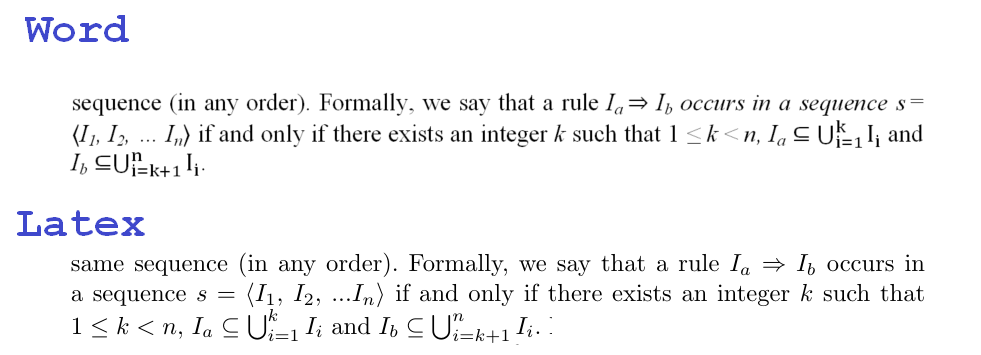
\includegraphics[width=1.0\linewidth]{images/word_vs_latex.png}
	        \caption{Fonte: \url{http://data-mining.philippe-fournier-viger.com}}
	        \label{latex_vs_word}
        \end{figure}
        
    \end{frame}
    
    \begin{frame}[fragile]{\sc \LaTeX \ vs Microsoft Word (eficiência)}
        
	    \begin{figure}[b!]
		    \centering
		    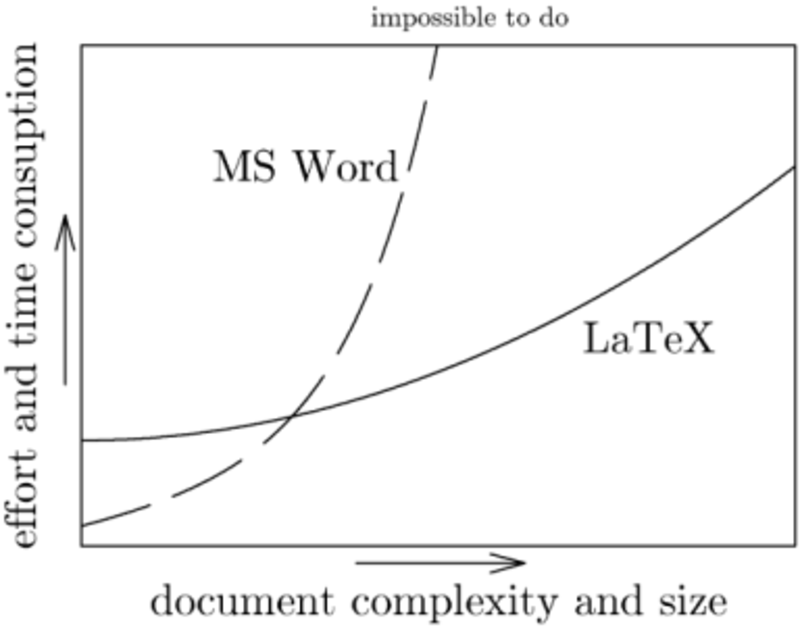
\includegraphics[width=0.7\linewidth]{images/wordvslatex.pdf}
		    \caption{Fonte: \url{https://www.johndcook.com/wordvslatex.gif}}
		    \label{latex_vs_word2}
	    \end{figure}
	    
    \end{frame}
    
\section{Instalação}
    
    \begin{frame}[fragile]{\sc Usuários Linux (recomendado)}
        
        \begin{itemize}
        \setlength\itemsep{0.2cm}
	        \item Instalando a biblioteca:
	        \begin{itemize}
                \item[$\to$] Abra o terminal (Ctrl+Alt+T) e digite:\\
                    \texttt{sudo apt install texlive-full}
            \end{itemize}
	        \item Instalando o compilador e visualizador de pdf:
	        \begin{itemize}
		        \item[$\to$] Há três compiladores muito usados:  TexStudio (recomendado), Kile e  TexMaker:\\
		            \texttt{sudo apt install texstudio} ou \texttt{kile} ou \texttt{texmaker}
    		    \item[$\to$] O TexStudio e o TexMaker possuem um visualizador embutido. Outras opções são Okular, FoxitReader ou AdobeReader;
		        \item[$\to$] Para instalar o okular:\\
		            \texttt{sudo apt install okular}
	        \end{itemize}
        \end{itemize}
        
    \end{frame}
    
    \begin{frame}[fragile]{\sc Usuários Windows}
        
	    Para a instalação do \LaTeX \ no Windows, basta fazer o download e instalação de:
	    \begin{itemize}
	    \setlength\itemsep{0.3cm}
		    \item[$\to$] Texmaker: \url{http://cluster.ft.unicamp.br/wiki/doku.php?id=ambiente:latex_windows};
		    \item[$\to$] Baixe a versão correta para seu computador;
		    \item[$\to$] Baixar o \TeX \ Live: \url{https://www.tug.org/texlive/acquire-netinstall.html} em \emph{install-tl-windows.exe}. \quad ($\sim$ 4.4 Gb)
	    \end{itemize}
	    
    \end{frame}

\section{Conhecendo o compilador}
    
    \subsection{TexStudio}
        
        \begin{frame}[standout]
            
            Vejamos o compilador TexStudio!
            
        \end{frame}

\section{Estrutura de um documento}

    \begin{frame}[fragile]{\sc Estrutura de um documento: preâmbulo e corpo}
        
	    Um documento (\verb|.tex|) em \LaTeX \ é composto, basicamente, de duas partes:
	    \begin{itemize}	
	    \setlength\itemsep{0.2cm}
		    \item {\color{blue} Preâmbulo}: contém todas as configurações do texto a ser criado, são feitas as declarações sobre a {\color{blue} classe} do documento, {\color{blue} configurações globais} e o carregamento dos {\color{blue} pacotes}. É possível criar somente um documento para este fim - o {\color{blue} documento mestre} (veremos adiante);
            \item {\color{blue} Corpo}: contém o texto propriamente dito.
	    \end{itemize}
	    
    \end{frame}

    \subsection{Preâmbulo}
        
        \begin{frame}[fragile]{\sc Preâmbulo: classe (\texttt{documentclass})}
        
	        \begin{itemize}
		    \setlength\itemsep{0.2cm}
		        \item A {\color{blue} classe} de um documento é o modelo de texto a ser criado:
		            \begin{verbatim}
    \documentclass[options]{class}
		            \end{verbatim}
                \item As {\color{blue} opções} se referem às seguintes configurações:
                \begin{itemize}
  	                \item[$\to$] Tamanho da fonte do texto (\verb|10pt|, \verb|12pt|, \verb|14pt|);
                    \item[$\to$] Formato do papel (\verb|a4paper|);
  	                \item[$\to$] Número de colunas (\verb|onecolumn|, \verb|twocolumn|);
  	                \item[$\to$] Orientação da folha (\verb|landscape|, \verb|portrait|);
  	                \item[$\to$] Impressão só frente ou frente e verso (\verb|oneside|, \verb|twoside|).
                \end{itemize}
            \end{itemize}
            
        \end{frame}
        
        \begin{frame}[fragile]{\sc Preâmbulo: classe (\texttt{documentclass})}
            
            Aguns tipos de classe são:
	        \begin{itemize}
	        \setlength\itemsep{0.2cm}
	            \item \verb|article|: Artigos científicos, documentos curtos, relatórios, etc;
	            \item \verb|beamer|: Apresentações \LaTeX;
	            \item \verb|book|: Livros;
	            \item \verb|letter|: Cartas;
	            \item \verb|report|: Livros pequenos, teses, relatórios longos, etc.
            \end{itemize}
            
        \end{frame}
        
        \begin{frame}[fragile]{\sc Preâmbulo: pacotes (\texttt{usepackage})}
            
	        \begin{itemize}
		    \setlength\itemsep{0.2cm}
		        \item Os {\color{blue} pacotes} são as ferramentas da base \TeX\ a serem {\color{blue} importados} de acordo com a {\color{blue} necessidade} do texto;
		        \item  A {\color{blue} declaração} dos pacotes é feita através do {\color{blue} comando}:
		            \begin{verbatim}
    \usepackage[options]{package}
		            \end{verbatim}
		        \item {\color{blue} Exemplos} de pacotes importantes:
                \begin{itemize}
    	            \item[$\to$] \verb|babel|: Pacote para {\color{blue} hifenização} automática e modificação das {\color{blue} regras tipográficas} do texto. Para usar português do Brasil, usamos \texttt{brazil} como opção;
    	            \item[$\to$] \verb|inputenc|: \emph{{\color{blue} Encoding}} utilizado na fonte do documento. Caracteres com {\color{blue} acentos} podem ser digitados diretamente no código fonte. As opções mais usadas são o \verb|utf8| e o \verb|latin1|;
    	            \item[$\to$] \verb|amssymb|, \verb|amsmath|: Habilitam alguns {\color{blue} caracteres} e {\color{blue} comandos matemáticos} especiais;
    	            \item[$\to$] \verb|geometry|: Pacote para configurar as dimensões das {\color{blue} margens} e {\color{blue} largura} da folha;
		            \item[$\to$] \verb|graphicx|: Utilizado para inserir {\color{blue} figuras}.
		        \end{itemize}
	        \end{itemize}
	        
        \end{frame}
    
    \subsection{Corpo}
        
        \begin{frame}[fragile]{\sc Corpo: \texttt{documment}}
            
	        \begin{itemize}
	        \setlength\itemsep{0.3cm}
                \item O {\color{blue} corpo do documento} consiste em tudo aquilo que está inserido entre os
        seguintes comandos:\\
                    \begin{center}
   	                    \verb|\begin{document}|\\
   	                    .\\
   	                    .\\
   	                    .\\
   	                    \verb|\end{document}|
   	                \end{center}
   	            \item Todos os capítulos, seções e subseções devem estar inseridos entre estes comandos; 
   	            \item O que for escrito após o fim do documento será ignorado pelo compilador.
            \end{itemize}
            
        \end{frame}
        
        \begin{frame}[fragile]{\sc Corpo: organização}
            
	        \begin{itemize}
    		\setlength\itemsep{0.3cm}
		        \item Se você for criar um texto grande, é ideal que se mantenha uma {\color{blue} organização dos arquivos}.
    	    	    \begin{center}
	    	    	    \underline{Quais arquivos?}
            		\end{center}
	        	\item Por exemplo, se for criado um documento com $X$ capítulos, a dica é criar para cada capítulo uma pasta e nessa coloque todos os arquivos referentes ao capítulo;
		        \item O mesmo se aplica para arquivos de figuras.
	        \end{itemize}
	        
        \end{frame}
        
        \begin{frame}[fragile]{\sc Corpo: organização}
            
	        \begin{itemize}
		    \setlength\itemsep{0.3cm}
		        \item Crie um {\color{blue} documento mestre}. Esse é constituído do preâmbulo com os pacotes $+$ o corpo, entretanto não escreva nenhum texto no corpo;
		        \item Ao invés, dentro do \verb|document| (que é o corpo) {\color{blue} importe os arquivos} que contém o {\color{blue} texto} utilizando os comandos \verb|\input{pasta_1/texto_1}| ou \verb|\include{pasta_1/texto_1}|;
		        \item Por exemplo:
		            \begin{verbatim}		
    \begin{document}
        \include{prefacio/prefacio}
        \input{capitulo_1/capitulo_1}
        \input{capitulo_2/capitulo_2}		
    \end{document}
		            \end{verbatim}
	        \end{itemize}
	        
        \end{frame}

\begin{comment}
        \begin{frame}[fragile]{\sc O pacote subfile}
            
            \begin{itemize}
            \setlength\itemsep{0.3cm}
                \item O pacote {\color{blue} \verb|subfile|}, assim como  {\color{blue}\verb|\input|} e  {\color{blue}\verb|\include|}, permite a modularização do documento.
                \item Para ser utilizado basta adicionar ao preâmbulo e chamar o arquivo com\\
                    \verb|\subfile{}|,\\
                    e o subarquivo deve conter\\
                    \verb|\documentclass[diretório do main/main.tex]{subfiles}|.\\
                \item Sua principal vantagem é que os subarquivos são arquivos \verb|.tex| o que permite sua compilação separada do arquivo principal, sem ser necessário compilar todos os documentos ao mesmo tempo
                \item Ideal para documentos grandes, como teses e livros, com multiplos capítulos.
                \item Sua principal desvantagem é que para que o pacote {\color{blue}\verb|graphicx|} funcione normalmente é necessário informar o diretório relativo das imagens em relação ao documento principal e ao subarquivo\\
                    \verb|\grapichspath{{images/}{../images}}|.
            \end{itemize}
            
        \end{frame}
\end{comment}        

\section{Formatação de texto}
    
    \subsection{Comandos de texto}
        
        \begin{frame}[fragile]{\sc Comandos de texto}
            
	        \begin{itemize}
            \setlength\itemsep{0.5cm}
	        	\item O \LaTeX é estruturado a base de {\color{blue} comados} e {\color{blue} sintaxes}, porém todos relativamente simples;
		        \item {\color{blue} Palavras} são separadas por espaços em branco;
		        \item Todo {\color{blue} comando} inicia com um \emph{{\color{blue} backslash}} \verb|\|;
                \item {\color{blue} Comentários} no editor são criados com \verb|%|. Qualquer caractere preenchido com \verb|%| não aparecerá no arquivo \verb|.pdf|;
		        \item {\color{blue} Caracteres especiais do \LaTeX}: \verb|%|, \verb|#|, \verb|&| e \verb|$|. Se quiser usá-los como texto, deve usar \verb|\| à esquerda, por exemplo \verb|\%|, etc;
		        \item Caracteres matemáticos são incluídos no texto entre dois símbolos \verb|$|.
	        \end{itemize}
	        
        \end{frame}
        
        \begin{frame}[fragile]{\sc O uso de \texttt{\$}}
            
	        \begin{itemize}
		    \setlength\itemsep{0.3cm}
		        \item O {\color{blue} símbolo \verb|$|} é utilizado para marcar {\color{blue} caracteres matemáticos} no texto:
	                \begin{table}[h]
		                \begin{tabular}{|c|}
		                    \hline
			                Seja $a$ e $b$ definidos pela relação: $a+b=1$.\\
			                \hline
			                \verb|Seja $a$ e $b$ definidos pela relação: $a+b=1$.|\\
			                \hline
			            \end{tabular}
	                \end{table}
	            \item Veremos mais sobre seu uso adiante.
            \end{itemize}
            
        \end{frame}
        
        \begin{frame}[fragile]{\sc Exercício de texto simples}
            
	        Reproduza o texto a seguir:\\[0.5cm]
	        
            ``O orçamento para 2017 [\dots] estava insuficiente para que tocássemos o ano com tranquilidade'', diz o presidente do CNPq, Mario Neto Borges. No total, o Orçamento previa R\$ 1,3 bilhão e o fundo, R\$ 400 milhões à autarquia - 44\% desses valores foram contingenciados. Do fundo, o CNPq recebeu menos do que 56\%: até o momento o valor pago foi R\$ 62 milhões.
            
            Fonte: Agência Brasil \href{http://agenciabrasil.ebc.com.br/educacao/noticia/2017-08/apos-corte-de-verbas-cnpq-tem-recursos-para-pagar-bolsas-apenas-ate-este}{(link)}
            
        \end{frame}
        
        \begin{frame}[fragile]{\sc Exercício de texto simples (solução)}
            
            \begin{verbatim}
                
``O nosso orçamento para 2017 [\dots] estava insuficiente
para que tocássemos o ano com tranquilidade'', diz o
presidente do CNPq, Mario Neto Borges. No total, o Orçamento
previa R\$ 1,3 bilhão e o fundo, R\$ 400 milhões à autarquia
- 44\% desses valores foram contingenciados. Do fundo, o CNPq
recebeu menos do que 56\%: até o momento o valor pago foi
R\$ 62 milhões.
            
			\end{verbatim}
			
        \end{frame}
        
    \subsection{Formatação e ajuste de texto}
        
        \begin{frame}[fragile]{\sc Formatação: justificação e hifenização}
            
	        \begin{itemize}
		    \setlength\itemsep{0.3cm}
		        \item No \LaTeX, o texto é {\color{blue} justificado automaticamente}; 
		        \item A opção \verb|brazil| do pacote \verb|babel| trata de {\color{blue} hifenizar automaticamente} as palavras para nova linha no idioma PT-BR.
	        \end{itemize}
	        
        \end{frame}
        
        \begin{frame}[fragile]{\sc Formatação: negrito, itálico, sublinhado e outros}
            
	        \begin{itemize}
		    \setlength\itemsep{0.3cm}
                \item {\color{blue} Negrito}: \verb|\textbf{Texto}| ou \verb|{\bf Texto }| produz \textbf{Texto};
                \item {\color{blue} Itálico}: \verb|\textit{Texto}| ou \verb|\emph{Texto}| produz \textit{Texto};
                \item {\color{blue} Sublinhado}: \verb|\underline{Texto}| produz \underline{Texto};
                \item {\color{blue} Letra de código}: \verb|\texttt{Texto}| produz \texttt{Texto};
                \item {\color{blue} Fonte \verb|sc|} para títulos: \verb|{\sc Título}| ou \verb|\textsc{}| produz {\sc Título};
                \item {\color{blue} Alterando a cor}: \verb|{\color{blue} Texto}| produz {\color{blue} Texto}.
	        \end{itemize}
	        
            OBS: Note o uso frequente de \verb|{}| para delimitar a região de atuação de um dado comando! Dessa maneira, \{ \} não é inserido no texto, para isso utilize \verb|\{ \}|.
            
        \end{frame}
        
        \begin{frame}[fragile]{\sc Formatação: tamanho e tipo da fonte}
            
	        \begin{itemize}
		    \setlength\itemsep{0.3cm}
		        \item o {\color{blue} tamanho do texto} é modificado de acordo com o apresentado abaixo:
	                \begin{table}[h]
		                \begin{tabular}{|c|c|}
			                \hline
			                \verb|{\tiny Texto}|            & {\tiny Texto}\\
			                \hline
			                \verb|{\scriptsize Texto}|      & {\scriptsize Texto}\\
			                \hline
			                \verb|{\footnotesize Texto}|    & {\footnotesize Texto}\\
			                \hline
			                \verb|{\small Texto}|           & {\small Texto}\\
			                \hline
			                \verb|{\normalsize Texto}|      & {\normalsize Texto}\\
			                \hline
			                \verb|{\large Texto}|           & {\large Texto}\\
			                \hline
			                \verb|{\Large Texto}|           & {\Large Texto}\\
			                \hline
			                \verb|{\LARGE Texto}|           & {\LARGE Texto}\\
                            \hline
			                \verb|{\huge Texto}|            & {\huge Texto}\\
			                \hline
			                \verb|{\Huge Texto}|            & {\Huge Texto}\\
			                \hline
		                \end{tabular}
	                \end{table}
	            \item Uma {\color{blue} generalização} para o tamanho e espaçamento (das linhas) é obtida com o comando \verb|{\fontsize{12pt}{10.0}\selectfont Texto}| (12 é o tamanho e 10 o espaçamento).
	            
		    \end{itemize}
		    
        \end{frame}
        
        \begin{frame}[fragile]{\sc Formatação: espaçamento}
            
            O \LaTeX \ manipula os {\color{blue} espaçamentos automaticamente}, porém nem sempre o documento compilado fica do formato desejado. Portanto, existem alguns comandos para {\color{blue} manipular os espaçamentos}.
	        \begin{itemize}
		    \setlength\itemsep{0.3cm}
                \item \verb|\hspace{tamanho}|: Produz espaçamento horizontal;
                \item \verb|\vspace{tamanho}|: Produz espaçamento vertical;
                \item \verb|\\[tamanho]|: Produz espaçamento vertical antes de começar uma nova linha.
            \end{itemize}
            
            Estes três comandos acima necessitam da {\color{blue} opção} \texttt{tamanho} que é definido pelo usuário. Esta opção deve ser um {\color{blue} número} seguido de sua {\color{blue} unidade}. Por exemplo,
            \begin{itemize}
		    \setlength\itemsep{0.3cm}
	            \item \verb| \hspace{5cm}|;
	            \item \verb| \\ [8mm]|.
	        \end{itemize}
	       
        \end{frame}
        
        \begin{frame}[fragile]{\sc Formatação: espaçamento}
            
	        Existem {\color{blue} outros comandos} que não necessitam de um tamanho especificado pelo usuário:
	        \begin{itemize}
	        \setlength\itemsep{0.3cm}
                \item \verb|\hfill|: Adiciona espaços horizontais para preencher a largura da página;
                \item \verb|\vfill|: Adiciona espaços verticais para preencher a altura da página;
                \item \verb|\newline|: Inicia uma nova linha;
                \item \verb|\newpage|: Inicia uma nova página;
                \item \verb|\noindent|: Remove o espaçamento antes do parágrafo.
            \end{itemize}
            
        \end{frame}
        
        \begin{frame}[fragile]{\sc Formatação: espaçamento}
            
            No \LaTeX \ também é possível modificar o {\color{blue} espaçamento entre linhas}. Há mais de uma forma de modificar este espaçamento. Para isto, teremos que adicionar ao preâmbulo o pacote
            \begin{verbatim}
    \usepackage{setspace}
            \end{verbatim}
            O espaçamento pode ser modificado utilizando os comandos
	        \begin{itemize}
		    \setlength\itemsep{0.3cm}
                \item \verb|\singlespacing|: Espaçamento simples entre linhas ;
                \item \verb|\onehalfspacing|: Espaçamento $1.5$;
                \item \verb|\doublespacing|: Espaçamento duplo.
	        \end{itemize}
	        
            Também é possível utilizar o comando
            \begin{verbatim}
    \renewcommand{\baselinestretch}{1.0}.
            \end{verbatim}
            (troque $1.0$ pelo espaçamento desejado!).
            
        \end{frame}
        
        \begin{frame}[fragile]{\sc Formatação: fontes}
            
	        \begin{itemize}
            \setlength\itemsep{0.3cm}
		        \item É possível {\color{blue} trocar} a fonte de todo documento. A troca é realizada com a adição do respectivo pacote de cada fonte.
		        \item Algumas fontes disponíveis que suportam o ambiente matemático são:
		            \begin{enumerate}[$\to$]
			            \item Padrão: \verb|cmr| (não é preciso pacote);
	                    \item Arev Sans: pacote \verb|arev|;
			            \item Garamond: pacote \verb|ebgaramond-maths|;
			            \item Palatino: pacote \verb|palatino|;
			            \item Times: pacote \verb|times|;
			            \item CM Bright: pacote \verb|cmbright|;
			            \item Concrete Font: \verb|ccfonts|;
			            \item Kurier: pacote \verb|kurier| com a opção \verb|math|;
		            \end{enumerate}
		            entre outros \footnote{Veja a lista completa em \url{http://www.tug.org/pracjourn/2006-1/hartke/hartke.pdf}}.
            \end{itemize}
            
        \end{frame}
    
    \subsection{Seccionando o documento}
        
        \begin{frame}[fragile]{\sc Hierarquia do documento: parte, capítulo, seções,...}
            
            Todo texto é organizado/dividido por {\color{blue} capítulos}, {\color{blue} seções}, etc, e essa {\color{blue} divisão} é {\color{blue} enumerada}. No \LaTeX, todas as enumerações são {\color{blue} automáticas} e essa é a grande vantagem. No \LaTeX, títulos e subtítulos são chamados de \texttt{section} e \texttt{subsection}.
            
            A {\color{blue} divisão hierárquica} completa é:
	        \begin{itemize}
		    \setlength\itemsep{0.3cm}
		        \item o 1º grau hierárquico de um documento é a parte: \verb|\part{Título da Parte}|;
		        \item o 2º grau hierárquico de um documento é o capítulo: \verb|\chapter{Título da Parte}| (é claro, exeto para classes que por definição não o possuem, por exemplo \verb|article|);
		        \item o 3º grau é a seção: \verb|\section{Seção 1}|;
		        \item o 4º grau é a subseção: \verb|\subsection{Subseção 1}|;
		        \item o 5º grau é a subsubseção: \verb|\subsubsection{Subsubseção 1}|;
		        \item o 6º grau é o parágrafo: \verb|\paragraph{Parágrafo 1}|.
	        \end{itemize}
            Para {\color{blue} remover a enumeração}, basta utilizar ``\verb|*|'' após o comando.
            
        \end{frame}
        
        \begin{frame}[fragile]{\sc Hierarquia do documento: parte, capítulo, seções,...}
            
            \center{Exemplo de títulos:}
            
            \vspace{0.2cm}
            
            \begin{columns}
	            \begin{column}{0.35\textwidth}
		            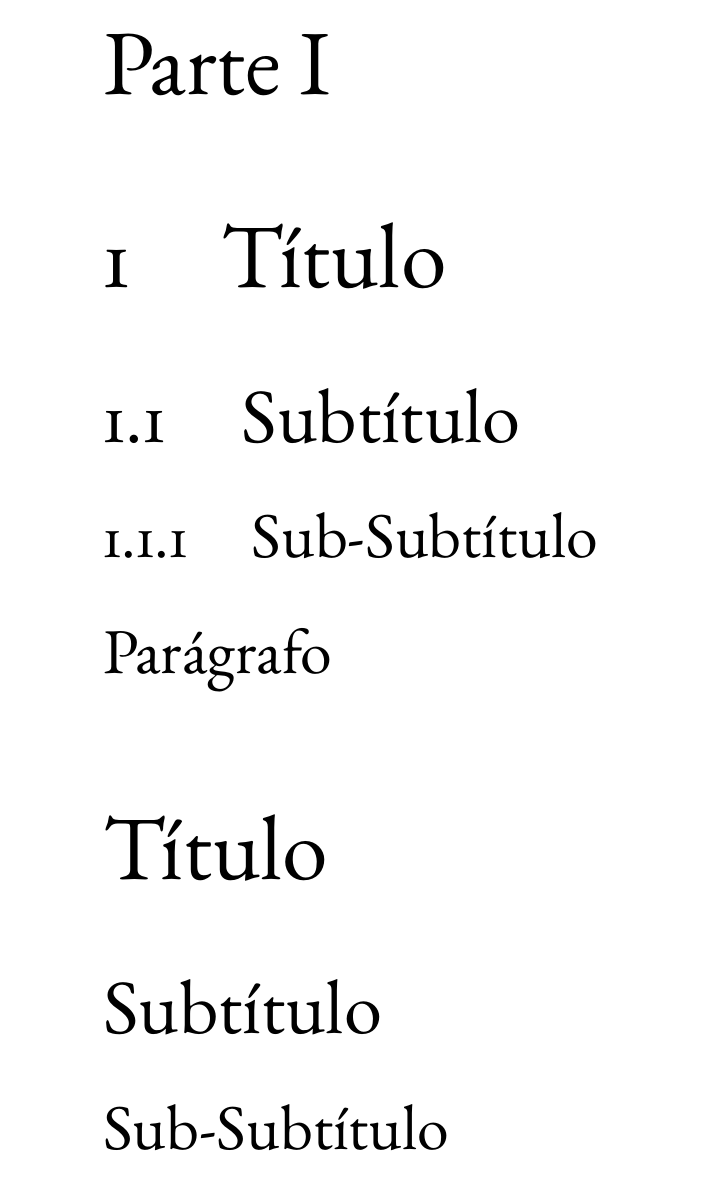
\includegraphics[scale=0.2]{images/exemplo_titulos.png}
		        \end{column}
		        \begin{column}{0.65\textwidth}
		            \begin{verbatim}
    \part{}
    \section{Título}
    \subsection{Subtítulo}
    \subsubsection{Sub-Subtítulo}
    \paragraph{Parágrafo}
    \section*{Título}
    \subsection*{Subtítulo}
    \subsubsection*{Sub-Subtítulo}
		            \end{verbatim}
		        \end{column}
			\end{columns}
        \end{frame}

\section{Exercício com a classe \texttt{article}}
    
    \begin{frame}[standout]
        
        O básico do \LaTeX\ já temos em mãos.\\
        Vamos começar a editar um texto simples!
        
    \end{frame}
    
    \begin{frame}[fragile]{\sc Exemplo \texttt{article}}
        
        \begin{verbatim}
    \documentclass[12pt,a4paper]{article}
    \usepackage[T1]{fontenc}
    \usepackage[brazil]{babel}
    \usepackage[utf8]{inputenc}
    \usepackage{amssymb,amsmath}
        \end{verbatim}
        
    \end{frame}

    \begin{frame}[fragile]{\sc Exemplo \texttt{article}}
        
        \begin{itemize}
	    \setlength\itemsep{0.5cm}
	        \item Após a importação dos pacotes, começamos editando o documento;
	        \item {\color{blue} Título} e {\color{blue} autor} são criados com \verb|\title{título}| e \verb|\author{autor}|, respectivamente;
	        \item A {\color{blue} data} é inserida automaticamente, caso contrário, use \verb|\date{data}| ou \verb|\date{\today}|;
	        \item Insira esses elementos após o \verb|\begin{document}|;
	        \item Para criar esses elementos no \verb|.pdf|, insira o comando \verb|\maketitle| logo em seguida.
        \end{itemize}
        
    \end{frame}
    
    \begin{frame}[fragile]{\sc Exercício \texttt{article}}
        
	    Como um exercício, crie um documento \verb|.tex| para a classe \verb|article|.
	    
	    \begin{itemize}
		\setlength\itemsep{0.3cm}
		    \item Adicione os pacotes a serem utilizados (copiem e colem o que já digitaram até agora);
		    \item Insiram as informações do título, autor e data;
		    \item Façam um pequeno texto, dividido por seções e subseções com o que foi aprendido até agora, formatação (negrito, itálico, tamanho, espaçamento, ...).
	    \end{itemize}
	    
    \end{frame}
    
    \begin{frame}[fragile]{\sc Exercício \texttt{article} (solução)}
        
        \begin{verbatim}
    \documentclass[12pt,a4paper]{article}
    \usepackage[T1]{fontenc}
    \usepackage[brazil]{babel}
    \usepackage[utf8]{inputenc}
    \usepackage{amssymb,amsmath}
    \usepackage{graphicx}
    
    \begin{document}
    
    \title{Minicurso de \LaTeX}
    \autor{Semana Acadêmica Integrada do IMEF}
    \date{\today}
    
    \maketitle
    
    texto a ser inserido aqui...
    
    \end{document}
        \end{verbatim}
        
    \end{frame}
    
\begin{frame}[standout]
    
    Fim do Módulo I!\\
    Dúvidas?
    
\end{frame}

\begin{frame}{Referências}
    
    \bibliography{references}
    \nocite{*}
    
\end{frame}

\begin{frame}[fragile]{\sc Links úteis}
    
    \Large{
	    Curso online de \LaTeX \ \href{https://www.overleaf.com/latex/learn/free-online-introduction-to-latex-part-1#.WZxOyXV97-c}{aqui}.\\[2cm]
	    
	    Livro extenso sobre \LaTeX \ \href{https://upload.wikimedia.org/wikipedia/commons/2/2d/LaTeX.pdf}{aqui}.
	}
	
\end{frame}

\begin{frame}[standout]
    
    \Huge{OBRIGADO! =)}
    
\end{frame}

}

\end{document}